\documentclass{phyasgn}
\phyasgn{
  stuname = 姚昊廷,           % 设置学生姓名
  stunum = 22322091,      % 设置学号
  setasgnnum = 6,           % 设置课程次数
  classname = 电动力学,     % 设置课程名称
}

\usepackage{listings}
\usepackage{tikz}
\usepackage{amssymb}
\usepackage{t-angles}
\usepackage{amssymb}
\usepackage{tikz}
\usepackage{mathrsfs}
\usepackage{pifont}
\usepackage{subfigure}
\usepackage{caption}
\usepackage{float}
%\usepackage{autobreak} 
%\usepackage{fixdif} 
\usetikzlibrary{quotes,angles}
\usetikzlibrary{calc}
\usetikzlibrary{decorations.pathreplacing}
\lstset{numbers=left,basicstyle=\ttfamily,columns=flexible}
\makeatletter
\newcommand{\rmnum}[1]{\romannumeral #1}
\newcommand{\Rmnum}[1]{\expandafter\@slowromancap\romannumeral #1@}
\renewcommand{\i}{\mathrm{i}}
\makeatother
\allowdisplaybreaks[4]%允许公式跨页


\begin{document}

\begin{sol}[1]
  设球外电势
  \begin{align*}
    \varphi=\frac{Q_f}{4\pi\varepsilon R}+\varphi'
  \end{align*}
  其中$\varphi'$是导体球表面电荷产生的电势,故在球外满足拉普拉斯方程
  \begin{align*}
    \nabla^2\varphi'=0
  \end{align*}  
  解得
  \begin{align*}
    \varphi'=\sum_{l=0}^{\infty}A_lr^{-l-1}+B_0
  \end{align*}
  因为无穷远处电势为0
  ,故$B_0=0$。
  代入球体表面边界条件有
  \begin{align*}
    (\frac{Q_f}{4\pi\varepsilon R}+\varphi')|_{r=R_0}&=0\\
    \frac{Q_f}{4\pi\varepsilon a}\sum_{l=0}^{\infty}(\frac{R_0}{a})^lP_l(\cos\theta)+\sum_{l=0}^{\infty}A_lR_0^{-l-1}&=0\\
  \end{align*}
  对比$P_l(\cos\theta)$系数得
  \begin{align*}
    A_l=-\frac{Q_fR_0^{2l+1}}{4\pi\varepsilon a^{l+1}}
  \end{align*}
  像电荷为$Q'=-\frac{R_0Q_f}{a}$,距球心$\frac{R_0^2}{a}$。故电像法得到的电势为
  \begin{align*}
    \varphi&=\frac{Q_f}{4\pi\varepsilon}(\frac{R_0}{aR_1}+\frac{1}{R_2})\\
    &=\frac{Q_f}{4\pi\varepsilon}(\frac{R_0}{a\sqrt{r^2+(\frac{R_0^2}{a})^2-2r\frac{R_0^2}{a}\cos\theta}}+\frac{1}{\sqrt{r^2+a^2-2ar\cos\theta}})
  \end{align*}
  展开为勒让德级数后与分离变量法得到的结果是一致的。
\end{sol}

\begin{sol}[2]
  像电荷大小为$-\frac{R_1}{a}Q$,距球心$\frac{R_1^2}{a}$。
  故电势为
  \begin{align*}
    \varphi=\frac{1}{4\pi\varepsilon_0}\left[\frac{Q}{\sqrt{r^2+a^2-2ar\cos\theta}}-\frac{QR_1}{a\sqrt{r^2+\frac{R_1^4}{a^2}-2\frac{2R_1^2r}{a}\cos\theta}}\right]
  \end{align*}
  由于导体球接地,故外壳电势为0,由唯一性定理可知球外无电场,故球壳外表面电荷为0.作一个半径在$R_1$,$R_2$之间的高斯球面可易知,感应电荷只分布在球壳内表面,且总量为$-Q$。
\end{sol}

\begin{sol}[3]
  球壳内部边界条件与上题相同,故内部电场强度一致,即内部电势至多相差一常数。

  当球壳有电势$\varphi_0$时,
  易知球壳内部电势为
  \begin{align*}
    \varphi=\frac{1}{4\pi\varepsilon_0}\left[\frac{Q}{\sqrt{r^2+a^2-2ar\cos\theta}}-\frac{QR_1}{a\sqrt{r^2+\frac{R_1^4}{a^2}-2\frac{2R_1^2r}{a}\cos\theta}}\right]+\varphi_0
  \end{align*}
  当球壳带电$Q_0$时,易知球壳电势为$\frac{Q+Q_0}{4\pi\varepsilon_0R_2}$,故球内电势为
  \begin{align*}
    \varphi'=\frac{1}{4\pi\varepsilon_0}\left[\frac{Q}{\sqrt{r^2+a^2-2ar\cos\theta}}-\frac{QR_1}{a\sqrt{r^2+\frac{R_1^4}{a^2}-2\frac{2R_1^2r}{a}\cos\theta}}\right]+\frac{Q+Q_0}{4\pi\varepsilon_0R_2}
  \end{align*}
  欲使
  \begin{align*}
    \varphi'=\varphi
  \end{align*}
  即
  \begin{align*}
    \varphi_0=\frac{Q+Q_0}{4\pi\varepsilon_0R_2}\\
  \end{align*}
\end{sol}

\begin{sol}[4]
  本题有三个像电荷,分别是$Q$与球面形成的像电荷$q_1$,$Q$与平面形成的像电荷$q_2$,$q_1$与平面形成的像电荷$q_3$。
  故
  \begin{align*}
    q_1&=-\frac{a}{b}Q\\
    q_2&=-Q\\
    q_3&=\frac{a}{b}Q
  \end{align*}
  以球心为原点,平面为$x-y$平面建立直角坐标系可以得到空间中电势为
  \begin{align*}
    \varphi&=\frac{Q}{4\pi\varepsilon_0}\Bigg(\frac{1}{\sqrt{x^2+y^2+(z-b)^2}}-\frac{1}{\sqrt{x^2+y^2+(z+b)^2}}\\
    &-\frac{a}{b\sqrt{x^2+y^2+\left(z-\frac{a^2}{b}\right)^2}}+\frac{a}{b\sqrt{x^2+y^2+\left(z+\frac{a^2}{b}\right)^2}}\Bigg)
  \end{align*}
\end{sol}

\begin{sol}[5]
  将两电极以一个小球面包围起来,故球面的电通量为
  \begin{align*}
    \iint_S\vec{E}\cdot\d \vec{S}&=\iint_S\frac{\vec{j}}{\sigma}\cdot\d \vec{S}\\
    &=\frac{1}{\sigma}\iint_S\vec{j}\cdot\d \vec{S}\\
    &=\frac{I}{\sigma}
  \end{align*}
  又由唯一性定理知道,这等效于一个电荷量为$Q$的电荷,且满足
  \begin{align*}
    \frac{I}{\sigma}&=\frac{Q}{\varepsilon_0}\\
    Q&=\frac{I\varepsilon_0}{\sigma}
  \end{align*}
  故会产生六个像电荷,空间中电势由这八个电荷叠加而成,故
  \begin{align*}
    \varphi&=\frac{I}{4\pi\sigma}\Bigg(\frac{1}{\sqrt{(x-x_0)^2+(y-y_0)^2+(z-z_0)^2}}-\frac{1}{\sqrt{(x-x_0)^2+(y-y_0)^2+(z+z_0)^2}}\\
    &+\frac{1}{\sqrt{(x+x_0)^2+(y-y_0)^2+(z+z_0)^2}}-\frac{1}{\sqrt{(x+x_0)^2+(y-y_0)^2+(z-z_0)^2}}\\
    &+\frac{1}{\sqrt{(x-x_0)^2+(y+y_0)^2+(z+z_0)^2}}-\frac{1}{\sqrt{(x-x_0)^2+(y+y_0)^2+(z-z_0)^2}}\\
    &+\frac{1}{\sqrt{(x+x_0)^2+(y+y_0)^2+(z-z_0)^2}}-\frac{1}{\sqrt{(x+x_0)^2+(y+y_0)^2+(z+z_0)^2}}\Bigg)
  \end{align*}
\end{sol}

\begin{sol}[6]
  \begin{figure}[H]
    \centering
    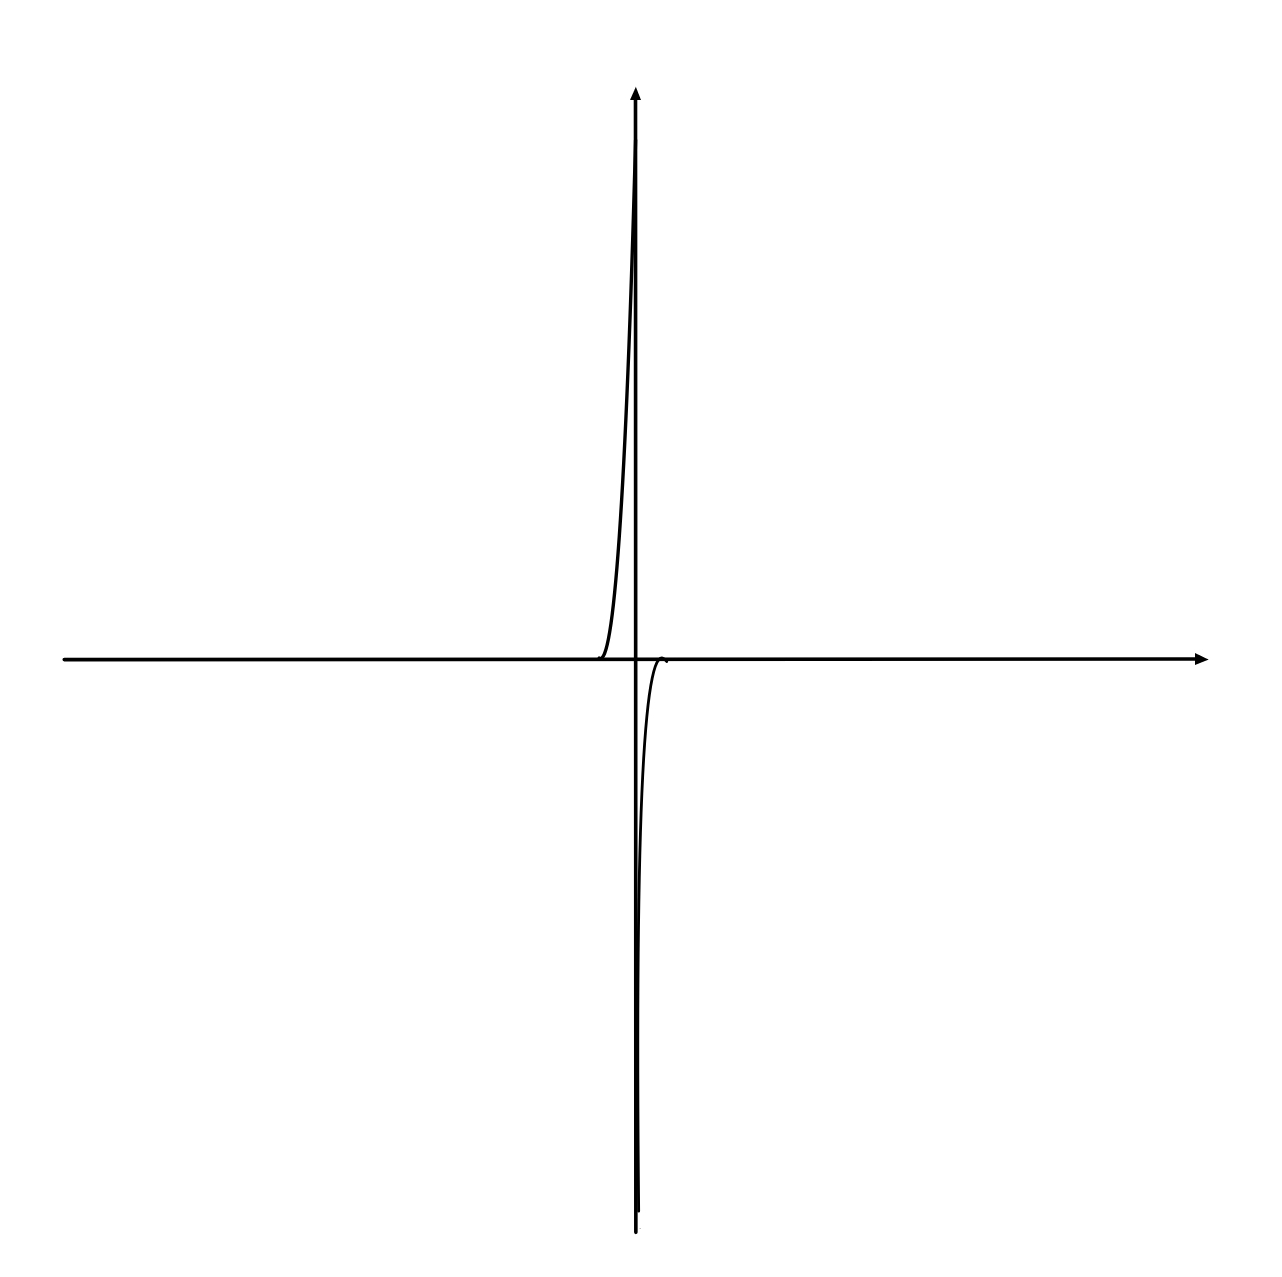
\includegraphics[width=0.5\textwidth]{狄拉克函数导数.jpg}
  \end{figure}
  不妨将$\vec{p}$的方向取为沿$x$轴正方向,则电偶极子的电荷密度可写为
  \begin{align*}
    \rho&=q\delta(x-\frac{l}{2})-q\delta(x+\frac{l}{2})\\
    &=-ql\frac{\delta(x+\frac{l}{2})-\delta(x-\frac{l}{2})}{l}
  \end{align*}
  取$l\to 0$的极限,则
  \begin{align*}
    \rho&=-ql\frac{\d \delta(x)}{\d x}
  \end{align*}
  故
  \begin{align*}
    \rho=-(p\cdot\nabla)\delta(x)
  \end{align*}
\end{sol}

\begin{sol}[7]
  定解条件为
  \begin{align*}
    \left\{\begin{matrix}
      \nabla^2\varphi_{in}=0\\
      \nabla^2\varphi_{out}=0\\
      \lim_{r\to\infty}\varphi_{out}=0\\
      \lim_[r\to0]\varphi_{in}\text{有限}
    \end{matrix}\right.
  \end{align*}
  故解得
  \begin{align*}
    \varphi_{out}&=\sum_{l=0}^{\infty}A_lr^{-l-1}P_l(\cos\theta)\\
    \varphi_{in}&=\sum_{l=1}^{\infty}B_lr^{l}P_l(\cos\theta)\\
  \end{align*}
  代入球体表面边界条件有
  \begin{align*}
    \sum_{l=0}^{\infty}A_lR_0^{-l-1}P_l(\cos\theta)&=\left\{\begin{matrix}
      \varphi_0(0<\theta<\frac{\pi}{2})\\
      -\varphi_0(\frac{\pi}{2}<\theta<\pi)
    \end{matrix}\right.\\
    \sum_{l=0}^{\infty}B_lR_0^{l}P_l(\cos\theta)&=\left\{\begin{matrix}
      \varphi_0(0<\theta<\frac{\pi}{2})\\
      -\varphi_0(\frac{\pi}{2}<\theta<\pi)
    \end{matrix}\right.
  \end{align*}
  解得
  \begin{align*}
    A_l&=\varphi_0R_0^{l+1}[P_{l-1}(0)-P_{l+1}(0)]\\
    B_l&=\frac{\varphi_0[P_{l-1}(0)-P_{l+1}(0)]}{R_0^l}
  \end{align*}
\end{sol}

\begin{sol}[7]
  格林函数可取为
  \begin{align*}
    G(r,\theta,\phi,r',\theta',\phi')=\frac{1}{4\pi\varepsilon_0}\left[\frac{1}{\sqrt{r^2+r'^2-2rr'\cos(\theta-\theta')}}-\frac{1}{\sqrt{(\frac{rr'}{R_0})^2+R_0^2-2rr'\cos(\theta-\theta')}}\right]
  \end{align*}
  故
  \begin{align*}
    \varphi=\varepsilon_0\int\limits_{r'=R_0}\varphi(R_0,\theta,\phi)\frac{\partial G}{\partial n}\d\vec{S}
  \end{align*}
  可记$\frac{r}{R_0}=R$,故最后结果为
  \begin{align*}
    \varphi&=\left\{\begin{matrix}
      -\frac{\varphi_0}{2}\left(\int_{0}^{\frac{\pi}{2}}-\int_{\frac{\pi}{2}}^{\pi}\right)\frac{R^2-1}{[1+R^2-2R\cos(\theta-\theta')]^\frac{3}{2}}\sin\theta'\d\theta'&R>1\\
      \frac{\varphi_0}{2}\left(\int_{0}^{\frac{\pi}{2}}-\int_{\frac{\pi}{2}}^{\pi}\right)\frac{R^2-1}{[1+R^2-2R\cos(\theta-\theta')]^\frac{3}{2}}\sin\theta'\d\theta'&R<1
    \end{matrix}\right.\\
    &=-\frac{\varphi_0}{2}\left(\int_{0}^{\frac{\pi}{2}}-\int_{\frac{\pi}{2}}^{\pi}\right)\frac{|R^2-1|}{[1+R^2-2R\cos(\theta-\theta')]^\frac{3}{2}}\sin\theta'\d\theta'
  \end{align*}
  这是一个椭圆积分,用勒让德级数展开后与上题结果一致。
\end{sol}
\end{document}